\documentclass[12pt,oneside]{uhthesis}
\usepackage{subfigure}
\usepackage[ruled,lined,linesnumbered,titlenumbered,algochapter,spanish,onelanguage]{algorithm2e}
\usepackage{amsmath}
\usepackage{amssymb}
\usepackage{amsbsy}
\usepackage{qrcode}
\usepackage{caption,booktabs}
\captionsetup{ justification = centering }
%\usepackage{mathpazo}
\usepackage{float}
\setlength{\marginparwidth}{2cm}
\usepackage{todonotes}
\usepackage{listings}
\usepackage{xcolor}
\usepackage{multicol}
\usepackage{graphicx}
\floatstyle{plaintop}
\restylefloat{table}
\addbibresource{Bibliography.bib}
% \setlength{\parskip}{\baselineskip}%
\renewcommand{\tablename}{Tabla}
\renewcommand{\listalgorithmcfname}{Índice de Algoritmos}
%\dontprintsemicolon
\SetAlgoNoEnd

\definecolor{codegreen}{rgb}{0,0.6,0}
\definecolor{codegray}{rgb}{0.5,0.5,0.5}
\definecolor{codepurple}{rgb}{0.58,0,0.82}
\definecolor{backcolour}{rgb}{0.95,0.95,0.92}

\lstdefinestyle{mystyle}{
    backgroundcolor=\color{backcolour},   
    commentstyle=\color{codegreen},
    keywordstyle=\color{purple},
    numberstyle=\tiny\color{codegray},
    stringstyle=\color{codepurple},
    basicstyle=\ttfamily\footnotesize,
    breakatwhitespace=false,         
    breaklines=true,                 
    captionpos=b,                    
    keepspaces=true,                 
    numbers=left,                    
    numbersep=5pt,                  
    showspaces=false,                
    showstringspaces=false,
    showtabs=false,                  
    tabsize=4
}

\lstset{style=mystyle}

\title{Metodología para la predicción del desempeño de un estudiante en un curso dentro de un Entorno Virtual de \\\vspace{0.25cm} Aprendizaje}
\author{\\\vspace{0.25cm}Jorge Alejandro Soler González}
\advisor{\\\vspace{0.25cm}MSc. Carmen Fernández Montoto\footnote[1]{Facultad de Matemática y Computación, Universidad de la Habana, Cuba}\\\vspace{0.25cm}MSc. Jorge Miguel Soler McCook\footnote[2]{Universidad Metropolitana del Ecuador, Ecuador}}
\degree{Licenciado en Ciencia de la Computación}
\faculty{Facultad de Matemática y Computación}
\date{Enero 2024\\\vspace{0.25cm}\qrcode[height=2cm]{https://github.com/jorgesolerrr/Student-behavior-prediction-and-recommendation-system}}
\logo{Graphics/uhlogo}
\makenomenclature

\renewcommand{\vec}[1]{\boldsymbol{#1}}
\newcommand{\diff}[1]{\ensuremath{\mathrm{d}#1}}
\newcommand{\me}[1]{\mathrm{e}^{#1}}
\newcommand{\pf}{\mathfrak{p}}
\newcommand{\qf}{\mathfrak{q}}
%\newcommand{\kf}{\mathfrak{k}}
\newcommand{\kt}{\mathtt{k}}
\newcommand{\mf}{\mathfrak{m}}
\newcommand{\hf}{\mathfrak{h}}
\newcommand{\fac}{\mathrm{fac}}
\newcommand{\maxx}[1]{\max\left\{ #1 \right\} }
\newcommand{\minn}[1]{\min\left\{ #1 \right\} }
\newcommand{\lldpcf}{1.25}
\newcommand{\nnorm}[1]{\left\lvert #1 \right\rvert }
\renewcommand{\lstlistingname}{Ejemplo de código}
\renewcommand{\lstlistlistingname}{Ejemplos de código}

\begin{document}

\frontmatter
\maketitle

\begin{dedication}
    Dedicación
\end{dedication}
%\begin{acknowledgements}
    Agradecimientos
\end{acknowledgements}
\begin{opinion}
    En los últimos años, en las instituciones educacionales existe una marcada tendencia hacia el uso de los Entornos Virtuales de Aprendizaje, los cuales permiten la propagación de su instrucción a mayor número de personas, apoyándose en las facilidades que ofrecen estas plataformas.  

En estos entornos se produce una gran cantidad de información valiosa referente al aprendizaje de los alumnos que no siempre es objeto de análisis por parte de la institución, el profesorado, incluso del estudiantado, en aras de lograr mejores resultados en su proceso de enseñanza-aprendizaje.  

La Minería de Datos Educacionales (MDE), es un campo de estudio que aporta un conjunto de técnicas que facilitan el análisis de grandes repositorios de datos generados o relacionados con las actividades de aprendizaje en los centros educativos, con el objetivo de orientar mejor el proceso de instrucción, evaluar el comportamiento del desempeño de sus estudiantes, desarrollar un mejor trabajo colaborativo en los educandos, entre otras muchas acciones proveniente del análisis efectuado.  

El trabajo de investigación que se aborda en esta tesis, parte del análisis de las técnicas de minería de datos que faciliten la extracción de la información educacional y a partir de ella poder realizar predicciones del comportamiento del desempeño que llevan los estudiantes de un determinado curso, en aras de facilitar el proceso de enseñanza-aprendizaje.  

El autor primeramente ha tenido que dedicar un tiempo considerable a profundizar en la plataforma Moodle desde el punto de vista usuario y desarrollador, profundizar en los registros necesarios para obtener la información necesaria para aplicar las técnicas de aprendizaje de máquina, determinar aquellas que se fueran mejores para establecer las posibles predicciones y brindarla a la institución para su posterior análisis para la toma de decisiones.  

Ha tenido que realizar un estudio del estado del arte para determinar el camino a seguir, así como profundizar en las estructuras de la plataforma para poder insertarse en el contexto de esta. Para ello, ha tenido que consultar diferentes bibliografías, en su mayoría en idioma inglés.  

En el desarrollo de esta tesis el estudiante evidenció su motivación por la investigación, la cual ha desarrollado de manera independiente, con profesionalidad, aportando sugerencias válidas para el desarrollo de la misma. Demostró el dominio alcanzado en los contenidos estudiados y los resultados alcanzados avalan la calidad de la plataforma instrumentada.  

Es de destacar la constancia y dedicación mostrada en el desarrollo de la investigación, así como las acciones que tuvo que desarrollar para recopilar los datos de los casos de estudios presentado, que no solo se redujo a los presentados en la memoria escrita.  

Consideramos que el autor posee las habilidades necesarias de un profesional en Ciencia de la Computación, evidenciándose en la aplicación de los conocimientos adquiridos al desarrollo de otras áreas del saber, por tales razones proponemos al tribunal se le otorgue la calificación de excelente (5).
\end{opinion}
\begin{resumen}
	Durante la pandemia de COVID-19, muchas universidades estuvieron en su mayor parte cerradas y sus aulas se transformaron 
	a un formato totalmente en línea. Para los profesores era un desafío gestionar el aprendizaje virtual y, especialmente, realizar 
	un seguimiento del comportamiento de los estudiantes, ya que no se podía establecer contacto interpersonal y por ende, el desempeño de los estudiantes no es fácil de controlar. Para aliviar 
	este problema, una solución, que se ha vuelto cada vez más importante, es la predicción del desempeño de los estudiantes en función 
	de sus datos históricos de registro en los entornos virtuales de aprendizaje. Este estudio, por tanto, tiene como objetivo analizar datos de comportamiento de los alumnos aplicando técnicas de aprendizaje automático a los registros de Moodle, con un total de $453941$ registros. Se utilizaron cinco algoritmos de aprendizaje automático 
	(\textit{Random Forest}, Árbol de Decisión, Regresión Logística, Regresión Lineal y \textit{Support Vector Machine}) para realizar la predicción académica. Además, se crearon dos conjuntos de datos con atributos distintos, los cuales se dividieron en cuatro etapas de progreso del curso 
	(25\%, 50\%, 75\% y 100\%), a los que se le aplicó un proceso de selección de características con el algoritmo Boruta.  

	Los modelos de predicción podría guiar estudios futuros, motivar la autopreparación y reducir las tasas de abandono. 
	En la investigación se evaluaron los modelos con validación cruzada quíntuple. Los resultados indicaron que en ambos conjuntos de datos el algoritmo de Regresión Lineal tuvo el mejor comportamiento en todas las etapas del curso.  

	Los resultados podrían aplicarse a otros cursos y en un registro más grande en entornos virtuales de aprendizaje que tengan condiciones similares de actividad de los estudiantes, en búsqueda de lograr una predicción más precisa del desempeño de los estudiantes.
\end{resumen}

\begin{abstract}
	During the COVID-19 pandemic, many universities were mostly closed, and their classrooms shifted to a fully online format. For teachers, managing virtual learning posed a challenge, especially in monitoring student behavior, as interpersonal contact was not possible, making it difficult to control student performance. To alleviate this problem, an increasingly important solution has been predicting student performance based on their historical log data in virtual learning environments.  

This study aims to analyze student behavior data by applying machine learning techniques to Moodle logs, totaling 453,941 records. Five machine learning algorithms (Random Forest, Decision Tree, Logistic Regression, Linear Regression, and Support Vector Machine) were used for academic prediction. Additionally, two datasets with different attributes were created, divided into four course progress stages (25\%, 50\%, 75\%, and 100\%), subjected to feature selection using the Boruta algorithm.  


The predictive models could guide future studies, motivate self-preparation, and reduce dropout rates. The research evaluated the models with five-fold cross-validation. The results indicated that in both datasets, the Linear Regression algorithm performed the best at all course stages.  


These findings could be applied to other courses and in a larger dataset in virtual learning environments with similar student activity conditions, aiming for a more accurate prediction of student performance.

\end{abstract}
\tableofcontents
\listoffigures
% \listoftables
% \listofalgorithms
%\lstlistoflistings

\mainmatter

\chapter*{Introducción}\label{chapter:introduction}
La formación de competencias profesionales es un aspecto fundamental en el proceso de instrucción en las 
instituciones educativas, principalmente en la educación superior y tecnológica. En la actualidad, 
gracias a los avances tecnológicos, el aprendizaje se ha vuelto más accesible y flexible a través de 
los Entornos Virtuales de Aprendizaje (EVA). Recientemente, la humanidad se encuentra aún dando 
solución a un problema global de pandemia que potenció la educación a distancia y todos sus mecanismos 
de enseñanza, por esta razón, la demanda de tecnología digital e innovadora para respaldar las tareas de 
enseñanza, administrar las clases y hacer un seguimiento de los alumnos se ha convertido en una parte 
crucial de la educación. [\cite{CrucialEdu}] 

En tiempos de pandemia la mayoría de los países fueron forzados a cerrar todas sus instituciones académicas 
y transitar al aprendizaje en línea. Aunque las clases virtuales eran portables, de fácil acceso 
y aumentaban las oportunidades de aprendizaje para adultos, todas las escuelas y universidades enfrentaron 
múltiples desafíos al requerir la adopción de programas de enseñanza no presencial.[\cite{Conferencia,Journal}] Muchos 
docentes y estudiantes, además, se encontraron con la difícil tarea de tener que continuar con sus cursos 
en este nuevo sistema, teniendo esto un impacto desfavorable en la calidad de algunos cursos. 

Dentro de los problemas más típicos que 
se pueden citar, está el hecho de que los estudiantes se pierden el trabajo de laboratorio y reciben 
menos retroalimentación porque con frecuencia son demasiado tímidos para hacer preguntas durante el curso, 
mientras que los profesores carecen de contacto directo en el aula con los estudiantes, no pueden 
observarlos ni explicar el contenido, y no pueden notificar de inmediato a los estudiantes que pueden 
estar en riesgo académico. Muchos de estos factores aumentan la probabilidad de que los estudiantes reprueben, 
abandonen y se retiren antes de graduarse. 

De igual manera, los entornos virtuales de aprendizaje han surgido como una valiosa 
herramienta en el ámbito educativo, se tornan indispensables en el contexto pandémico
que ha afectado a la humanidad. Estos entornos ofrecen a los estudiantes una 
experiencia de aprendizaje flexible y accesible, permitiéndoles adquirir 
conocimientos y desarrollar habilidades de manera eficiente y autónoma. Además, 
han demostrado su capacidad para adaptarse a las necesidades individuales de los 
estudiantes, brindando la oportunidad de personalizar los contenidos y el ritmo 
de aprendizaje. A medida que la sociedad se adentra en una nueva era digital, 
los entornos virtuales de aprendizaje se han consolidado como una solución 
duradera y eficaz, que no solo ha llegado para quedarse, sino que continuará 
evolucionando y transformando la forma en que enseñamos y aprendemos.

Las universidades, para seguir con esta dinámica, deben proporcionar herramientas de aprendizaje en línea para apoyar la educación 
de manera eficiente. En este sentido [\cite{Moodle_Solutions}], Moodle LMS(\textit{Moodle Learning Management System})
ofrece un entorno de aprendizaje con software digital, de libre acceso y además, de código abierto, de amplia utilización en muchas universidades del mundo, en el cual los estudiantes obtienen acceso rápido y eficiente a los recursos y actividades 
de un curso, mientras los profesores pueden usarlo como una herramienta eficiente para administrar el 
aula a través de cuestionarios, tareas, exámenes y otras actividades. Adicionalmente esta plataforma permite recopilar datos 
de la actividad estudiantil y docente, generando un archivo de registros de acceso bastante extenso. Esta última ventaja 
se puede utilizar para el análisis y el pronóstico del rendimiento de un estudiante dentro de un curso. Por todas estas 
características esta investigación se centra en cursos impartidos en esta plataforma.

En estos entornos virtuales de aprendizaje como Moodle es un reto para los profesores obtener una métrica que permita analizar 
y predecir el desempeño de cada estudiante durante un curso en el logro de los objetivos y habilidades
de estudio. Con esta investigación se busca desarrollar una herramienta que permita proveer, a tiempo, una 
atención personalizada a los estudiantes, logrando una intervención oportuna que permitiría conducir y 
afianzar la confianza de los estudiantes dentro del curso, a pesar de las brechas detectadas, en los resultados al 
finalizar este.

¿Qué facilita predecir el desempeño de un estudiante durante el curso?
\begin{itemize}

    \item Entender el aprendizaje académico del estudiante en su trayectoria en cada objetivo 
    académico dentro del entorno: esto, además, incluye el cómo está progresando hacia la consecución de 
    los objetivos académicos específicos del curso. Esto permite a los profesores y tutores identificar 
    áreas en las que el estudiante puede estar estancado y proporcionar intervenciones específicas para 
    ayudarles a mejorar su rendimiento. Además, también puede ayudar a identificar las fortalezas del 
    estudiante y permitir que se les brinden oportunidades para desarrollarlas aún más.

    \item Facilitar a los profesores entender las condiciones y realidades académicas 
    en las que están sus estudiantes, esto incluye factores como la carga de trabajo del estudiante, y otros factores que pueden influir en su 
    rendimiento académico. Al comprender mejor estas condiciones y realidades, los profesores 
    pueden ajustar su enseñanza y proporcionar apoyo personalizado para ayudar a los estudiantes 
    a alcanzar las habilidades requeridas.

    \item Implementar planes personalizados de recomendación. Una vez que se ha realizado la predicción 
    del rendimiento del estudiante, se pueden implementar planes personalizados de recomendación para 
    ayudar a mejorar su rendimiento. Estos planes pueden incluir guías específicas 
    para el estudio, la práctica y la preparación para exámenes, así como para el apoyo académico adicional, 
    como tutorías o asesoramiento individualizado.

\end{itemize}

Una forma de detectar a los estudiantes que pudieran tener un desempeño medio o bajo dentro de un curso, 
es realizar predicciones tempranas de sus calificaciones en los diferentes temas que se abordan.

El uso de modelos de predicción para el análisis del aprendizaje, así como los sistemas de recomendación, 
presentan múltiples desafíos, especialmente el cómo obtener, procesar y usar los datos para construir el modelo de 
predicción apropiado. A este campo dentro de la analítica del aprendizaje se le llama: Minería de datos educacionales. 
En este estudio se proponen los siguientes indicadores, los cuales son extraídos del archivo de registros de Moodle: 
\begin{itemize}
    \item Cantidad de veces que el estudiante ha ingresado a las actividades y recursos de la plataforma.
    \item Nivel de participación en los tipos diferentes de actividades.
    \item Resultado de la evaluación que se otorga por el docente en cada actividad interactiva de cada objetivo académico.
\end{itemize}

Este preprocesamiento de los datos a realizarse en esta investigación tiene significativa importancia puesto que 
interviene directamente en la precisión y en el costo computacional del modelo predictivo a emplear.

Luego, ¿Sería posible establecer un modelo de predicción y un sistema de recomendación en los 
Entornos Virtuales de Aprendizaje que facilite el proceso de enseñanza con el aprendizaje personalizado de los 
estudiantes en los cursos montados en la plataforma de una institución? 
En el contexto de la presente tesis, el objetivo general es responder a la interrogante anterior desarrollando 
un modelo predictivo y un sistema de recomendación a partir de los datos extraídos y preprocesados de Moodle. 

Como resultado de este trabajo se pretende predecir el comportamiento de un estudiante en un 
curso y, a partir de ella, se busca ofrecer recomendaciones personalizadas adaptadas a las 
necesidades y preferencias individuales de cada estudiante, con el fin de mejorar su 
desempeño en el proceso de aprendizaje y aumentar su rendimiento académico.

Para lograr este objetivo se tendrán en cuenta los siguientes objetivos específicos:
\begin{enumerate}
    \item Estudiar de la arquitectura de almacenamiento de la plataforma Moodle, dígase: Bases de datos, APIs de acceso a la información,
          descargas de archivos, etc. De donde se extraería la información sobre las actividades realizadas por los estudiantes y sus evaluaciones.
    \item Recopilar y procesar los datos pertinentes.
    \item Construir el modelo predictivo: Implementación de algoritmo de clasificación de aprendizaje de máquina.
\end{enumerate}

Este trabajo consta de 3 capítulos:
\begin{enumerate}
    \item Marco teórico-conceptual.
    \item La Propuesta.
    \item Detalles de Implementación y Resultados.
\end{enumerate}

\addcontentsline{toc}{chapter}{Introducción}



\chapter{Estado del Arte}\label{chapter:state-of-the-art}

\chapter{Propuesta}\label{chapter:proposal}

\section{Antecedentes}

Como ya se ha mencionado la educación a distancia ha experimentado un crecimiento significativo en los últimos años, y con ese crecimiento la necesidad de soluciones innovadores a los diferentes problemas que se presentan dentro de este campo, uno de los problemas más comunes es el abandono y el bajo rendimiento de los estudiantes en los cursos virtuales, este problema puede estar influenciado por varios factores, pero sin duda uno de ellos es la poca enseñanza personalizada que existe hoy en día en esa modalidad de enseñanza, lo que conlleva a un desinterés por parte del estudiante a la hora de abordar un curso.  


Históricamente la forma de lograr una enseñanza personalizada en la educación tradicional, es basada en la percepción que puede tener el docente dentro de un aula, pero en la educación distancia cambia porque los profesores no ven continuamente a sus estudiantes. Por lo tanto, lograr una predicción temprana del rendimiento que pueda tener un estudiante dentro de un curso virtual pasa a ser una parte crucial en el camino de evitar el abandono o el desinterés en el curso por parte de los estudiantes, ya que esto permite una toma de medidas temprana para ayudar a ese grupo de estudiantes que están potencialmente en riesgo.  

 
La educación virtual, y su influencia en el rendimiento académico de los estudiantes puede ser tanto positiva como negativa, dependiendo de la calidad de la instrucción y la adaptación a la modalidad virtual. Moodle puede proporcionar una experiencia de aprendizaje enriquecedora y efectiva si se utiliza adecuadamente, pero también puede ser un obstáculo si no se adapta correctamente a las necesidades de los estudiantes. Por lo tanto, es importante lograr tener cursos atractivos y de fácil manejo por los estudiantes, utilizando las diferentes herramientas de Moodle, logrando así un curso verdaderamente interactivo donde el estudiante se sienta motivado, ya que esto influye directamente en el rendimiento académico del estudiante.  


Identificar a los estudiantes que tienen más probabilidades de tener dificultades, se pueden tomar medidas preventivas para mejorar su rendimiento y reducir la tasa de deserción. De similar manera, si se identifica las mejores prácticas para perfeccionar el rendimiento académico de los estudiantes, estas se pueden implementar en otros cursos para mejorar la calidad de la enseñanza-apredizaje, la cual se logra mediante la integración de \textit{plugins} desarrollados por los programadores, con el objetivo de poder utilizar la herramienta en los cursos venideros.  

 
Para analizar y predecir el desempeño de los estudiantes en cursos virtuales, es necesario desarrollar modelos predictivos de rendimiento académico, utilizando datos generados en la gestión educativa y aplicando técnicas de aprendizaje automático. Estos modelos pueden ayudar a identificar a los estudiantes que tienen más probabilidades de tener dificultades y proporcionar apoyo adicional, por parte del docente, para mejorar su rendimiento; así como identificar las mejores prácticas para elevar el rendimiento académico de los estudiantes más sobresalientes y con ello mejorar la calidad del proceso enseñanza-aprendizaje, en los EVA.  


\section{Contexto del estudio}

A partir del 2021 los procesos educacionales se vieron afectados por la pandemia de COVID-19 producto del aislamiento interpersonal que sufrió la humanidad por casi dos años, a partir de ello las instituciones educacionales tuvieron que cambiar drásticamente su modalidad hacia la forma de enseñanza en línea o virtual, la cual ha llegado para quedarse. Por esta razón la demanda de tecnología digital innovadora se ha convertido en una parte crucial de la educación para respaldar las tareas docentes, educativas, el aprendizaje auto-gestionado y colaborativo, gestionar el proceso enseñanza aprendizaje mediado por las tecnologías, así como y  realizar un seguimiento personalizado de los alumnos en el proceso de compresión y asimilación de los contenidos y las habilidades alcanzadas en  cada curso matriculado.  


La tendencia hacia un aprendizaje centrado en el estudiante y que responda a sus necesidades ha aumentado de manera significativa el uso de entornos virtuales de aprendizaje. En este sentido, como se explicó en el capítulo anterior, Moodle es una plataforma que ofrece un ambiente ideal para llevar a cabo este enfoque, debido a sus potencialidades para la gestión de contenidos y la interrelación entre docentes y estudiantes, lo cual ha provocada su amplia utilización en los centros educacionales.  


Ejemplos del uso expansivo de esta plataforma se pueden citar los centros de altos de estudio asociados al Ministerio de Educación Superior de Cuba, La Universidad Metropolitana del Ecuador, Universidad de Barcelona,  Universidad de Harvard, entre otras muchas a nivel internacional.   


Para este estudio se utilizaron datos brindados por la Universidad Metropolitana del Ecuador, que posee un sistema de educación a distancia en Moodle desde el 2018, y que a partir de la pandemia se hizo mucho énfasis en esta modalidad de enseñanza y desde el 2020 se implementa un calendario por períodos, donde se imparten todo tipo de cursos. Los datos a los que se tuvieron acceso pertenecen a los cursos de grado de aprobación regular del primer semestre del 2023, en total son 401 cursos, con 453941 registros de actividad desde el inicio del período el 2 de abril del 2023 hasta el 1ro de julio del 2023. El archivo de registros proporcionado se muestran en la Figura \ref{Logs} 
\begin{figure}[htb]
    \centering
    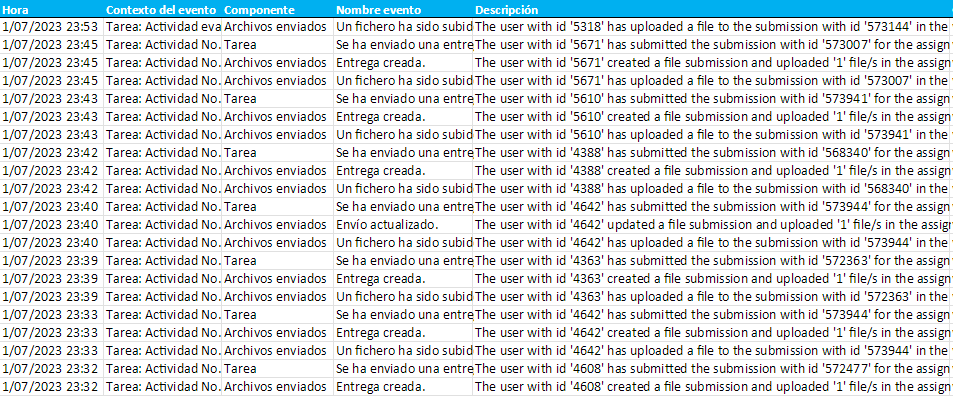
\includegraphics[width = 1 \textwidth]{Graphics/Pasted image 20231227101635.png}
    \caption{Muestra del archivo de registros proporcionado por la mencionada universidad}
    \label{Logs}
\end{figure}

En estos registros también se encuentran eventos realizados por los profesores, pero para la finalidad de esta investigación solamente se tienen en cuenta las actividades relacionadas con los estudiantes.  


Los 401 cursos se filtraron por los cursos que tuvieran bien establecido el libro de calificaciones de Moodle, que es lo que proporciona la nota final del estudiante dentro del curso. Se asume que el estudiante que tenga una nota por debajo de los 70 puntos su desempeño fue insatisfactorio. Finalmente se utilizaron 271 cursos, con un total de 2885 estudiantes.  


Las actividades y recursos dentro de un curso se les llama módulos, atendiendo a los datos facilitados de la universidad antes mencionada, se tuvo en cuenta los módulos más utilizados por los estudiantes, se llega a la conclusión de utilizar los registros relacionados con los siguientes tipos de módulos:   
\begin{itemize}
    \item Tarea
    \item Glosario
    \item Foro
    \item Cuestionario
    \item Carpeta
    \item Recurso
    \item URL
\end{itemize}
    
En el epígrafe 2.3 se verá la propuesta de procesamiento de datos llevada a cabo.  

\section{Propuesta de procesamiento de datos}

En esta tesis se presentan técnicas de análisis predictivo para la investigación de los datos referentes al comportamiento estudiantil. Se cuentan con 453.941 registros obtenidos de la plataforma Moodle de la mencionada institución universitaria. El objetivo es lograr predecir el desempeño académico de los estudiantes en las etapas del curso y hacer una comparación en el rendimiento de los diferentes modelos de aprendizaje automático utilizados (\textit{Random Forest}, Árboles de Decisión, regresión logística, regresión lineal y \textit{Support Vector Machine}).   


El diseño para la predicción se dividió en cuatro etapas fundamentales como se muestra en la figura \ref{Etapas}:
\begin{figure}[htb]
    \centering
    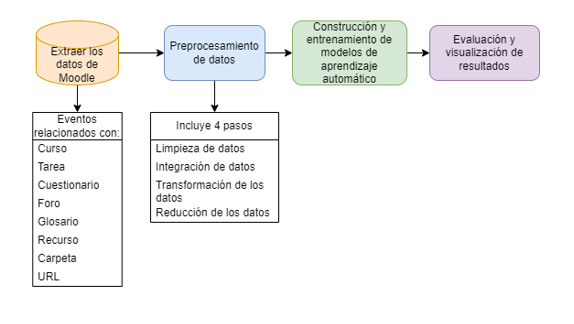
\includegraphics[width = 1 \textwidth]{Graphics/Pasted image 20240103010810.png}
    \caption{Etapas de la investigación}
    \label{Etapas}
\end{figure}

A continuación se expone la propuesta de solución en cada etapa.

\subsection{Recopilación de datos de Moodle}

Para el proceso de predicción se necesitan los datos de interacción de los estudiantes con la plataforma, así como la calificación del estudiante en cuestión, dentro del curso donde ha matriculado. Para esto Moodle cuenta con la opción de exportar un archivo de registros donde se encuentran todas las acciones realizadas dentro de los cursos que se quieran analizar. Este archivo de registros cuenta con la información tanto de estudiantes como de docentes. En el presente trabajo solo se abordan usuarios con rol de estudiante.  


Una vez obtenidos los registros, se necesita contrastar las acciones llevadas a cabo por los estudiantes con el desempeño obtenido en el curso con la nota final alcanzada. Las calificaciones obtenidas por un estudiante en un curso están organizadas en una estructura de categorías evaluativas a las que pertenecen las diferentes actividades. La organización de estas categorías y la relación y la formulación entre los resultados alcanzados en las mismas es lo que se denomina: el libro de calificaciones en Moodle.  


Luego ¿ cómo funciona el libro de calificaciones en Moodle ? Dentro de un curso existen varias etapas con objetivos a cumplir. Esas etapas se pueden entender como cortes parciales dentro de un curso. Dentro del libro de calificaciones estos cortes parciales se representan por categorías evaluativas, a estas categorías se le definen el peso que tendrá la nota alcanzada por el estudiante en ese corte parcial, con respecto a la nota total. Toda actividad dentro de una categoría de evaluación tiene un peso dentro de esa categoría.  


\begin{center}
    $NT = \displaystyle\sum_{i=1}^{m}PC_iNC_i$
\end{center}

Donde:  
\begin{itemize}
    \item $NT$ = Nota total
    \item $m$ = Número de cortes parciales
    \item $PC_i$ = Peso asignado a cada corte parcial (El examen final debe estar categorizado como un corte parcial, para que tenga su peso asignado)
    \item $NC_i$ = $\displaystyle\sum_{j=1}^{k}PA_jNA_j$ donde:
    \begin{itemize}
        \item $PA_j$ = Peso asignado a cada actividad dentro del corte parcial $i$
        \item $NA_j$ = Nota alcanzada en cada actividad
    \end{itemize}
\end{itemize}  

Para este trabajo se analizaron los cursos que cumplen con la fórmula anterior, es decir, todas sus actividades están categorizadas y es posible calcular la nota final del estudiante mediante esta fórmula.  


Para extraer estos datos se utiliza la API proporcionada por Moodle que permite el acceso a toda la información que se registra en esta plataforma. Como mecanismo de seguridad para realizar los llamados a las funciones que permiten obtener estos datos, se utiliza un \textit{token} de acceso que se gestiona con el rol de administrador de la plataforma. Estas funciones gestionan (obtener, modificar, crear o eliminar) cualquier módulo, curso o usuario de Moodle. En este estudio se utilizaron las siguientes funciones:  


\begin{itemize}
    \item \texttt{gradereport\_overview\_get\_course\_grades} : A partir del id de un usuario, devuelve las calificaciones finales de todos los cursos en los que ha participado.
    \item \texttt{gradereport\_user\_get\_grade\_items} : A partir del id de un curso y el id de un usuario, devuelve el libro de calificaciones asociado.
    \item \texttt{core\_enrol\_get\_enrolled\_users} : A partir del id de un curso, devuelve los usuarios matriculados en dicho curso y el rol con asignado.
    \item \texttt{core\_course\_get\_contents} : A partir del id de un curso, devuelve el contenido del curso, dividido por secciones y módulos.
    \item \texttt{core\_course\_get\_courses\_by\_field} : A partir de un campo determinado, se obtiene el id de un curso.
\end{itemize}
    
Con el acceso al API de Moodle, para cada curso se extrae toda la información relativa a su contenido (todo tipo de módulos a través de los cuales el docente establece un recurso o actividad en su curso), matrícula y las calificaciones otorgadas a cada estudiante. Las funciones utilizadas para obtener este tipo de información son de solo lectura garantizando la posibilidad de construir una herramienta, que incluso pueda repetir varias veces el proceso de investigación, sin correr el riesgo de que se modifique ningún registro del LMS. El resultado que que se obtiene en cada función del API se recibe en el formato JSON y esa respuesta se interpreta y se almacena para su posterior integración con el archivo de registros extraído de Moodle y de conjunto crear el \textit{dataset}. 

La cantidad de cursos influye en el tiempo de duración para el proceso de extracción de los datos, ya que por cada curso hay que hacer un conjunto de llamados a la API. Cada llamado tiene un costo de conexión a una base de datos remota y a la obtención de información mediante consultas de un volumen importante y creciente de información. Para resolver esta problemática se utilizaron técnicas de programación en paralelo, de manera que se puedan realizar las mismas operaciones en diferentes hilos. Con estas acciones se optimizó el tiempo de prospección de datos de 45 minutos en modo secuencial a 12 minutos en paralelo.
\subsection{Preprocesamiento de los datos}

El propósito de preprocesar los datos es filtrarlos para su posterior análisis y modelado. El proceso de limpieza y conversión de datos sin procesar que conducen al procesamiento y al análisis se conoce como ``preparación de datos''. Es una fase vital antes de procesar los datos que normalmente implica reformatearlos, realizar correcciones e integrar fuentes para aclararlos. En este estudio se crearon dos \textit{datasets} con atributos diferentes y se analizaron todos los modelos con ambos conjuntos de datos. 

Dentro del archivo de registros de Moodle vienen, entre otras cosas, la fecha en que ocurrió la interacción. Conociendo la duración del curso (en este caso todos tienen la misma duración, que coincide con la duración del período académico) , se dividieron ambos \textit{datasets} en cuatro nuevos conjuntos, uno con el 25\% del curso, otro con el 50\%, otro con el 75\% y otro con el 100\% del curso, se analizaron todos los algoritmos en cada uno de los \textit{datasets} con el objetivo de encontrar el mejor modelo de predicción para cada etapa del curso.

El primer conjunto de datos está hecho desde un punto de vista más general del estudiante. Se reunieron todas las interacciones por cada uno de los eventos relacionados con los módulos mencionados en la figura \ref{Etapas}. Cada estudiante es un vector, donde cada componente es un número natural que expresa el total de interacciones correspondiente al atributo de esa componente, los atributos son los siguientes: 

\begin{itemize}
    \item Tarea
    \item Glosario
    \item Cuestionario
    \item Foro
    \item Carpeta
    \item Recurso
    \item URL
    \item Estado : Si está aprobado o no.
\end{itemize}

Este conteo se logra a partir del campo \textbf{Componente} dentro del archivo de registros de Moodle, el cual asocia cada interacción con el módulo correspondiente. En este \textit{dataset} no se tiene en cuenta el evento relacionado con este módulo.  


El segundo conjunto está hecho teniendo en cuenta aspectos mucho más específicos de las interacciones. Los registros de cada uno de los atributos vistos en el \textit{dataset} anterior se dividen en nuevos atributos relacionados con el módulo en cuestión, logrando así una visión más detallada del comportamiento del estudiante. En este \textit{dataset} se tendrá en cuenta el campo \textbf{Evento} del archivo de registros.  Se realiza de la siguiente manera:  
\begin{itemize}
    \item Tarea : Se contabilizan por separado los eventos de vista y entrega de una tarea, añadiendo los siguientes atributos:
    \begin{itemize}
        \item Vista de Tarea: Asociado al módulo \textbf{Tarea} y al evento \textbf{Módulo de curso visto}.
        \item Entrega de Tarea: Asociado al módulo \textbf{Tarea} y al evento \textbf{Se ha enviado una entrega}.
    \end{itemize}
    \item Cuestionario: Se contabilizan por separado los eventos de vista, envío e intento, añadiendo los siguientes atributos:
    \begin{itemize}
        \item Vista de Cuestionario: Asociado al módulo \textbf{Cuestionario} y al evento \textbf{Módulo de curso visto}.
        \item Intento de Cuestionario: Asociado al módulo \textbf{Cuestionario} y al evento \textbf{Ha comenzado el intento}.
        \item Entrega de Cuestionario: Asociado al módulo \textbf{Cuestionario} y al evento \textbf{Intento enviado}.
    \end{itemize}
    \item Foro: Se contabilizan por separado las vistas del foro y la participación en este, añadiendo los siguientes atributos:
    \begin{itemize}
        \item Vista de Foro: Asociado al módulo \textbf{Foro} y al evento \textbf{Módulo de curso visto}.
        \item Participación en Foro: Asociado al módulo \textbf{Foro} y a los eventos \textbf{Tema creado}, \textbf{Algún contenido ha sido publicado}, \textbf{Mensaje actualizado}, \textbf{Mensaje creado}, \textbf{Suscripción activada}.
    \end{itemize}
\end{itemize}

Lo relacionado con los demás módulos (Recurso, Carpeta y URL) se mantiene igual al \textit{dataset} anterior, porque el único evento asociado con ellos es \textbf{Módulo de curso visto}, por lo tanto lo que se contabiliza en cada uno son las vistas. Además, se añadieron 2 nuevos atributos al \textit{dataset} que tienen que ver con las fechas de acceso por los estudiantes:
\begin{itemize}
    \item TAD: \textit{total access days} por sus siglas en inglés, se cuenta cada día (único) en el que el estudiante realizó una acción en la plataforma.
    \item ADS: \textit{access density score} por sus siglas en inglés, se calcula a partir de la división entre el TAD y el total de días que dura el curso, logrando de esta manera una métrica del esfuerzo hecho por el estudiante.
\end{itemize}

Esta idea viene del estudio [\cite{Jennifer}] donde utilizan esas variables en su \textit{dataset}, logrando un mejor análisis de lo que sucede con el estudiante en la plataforma. Además, por cuestiones de experimentación se añadieron 4 nuevas variables que describen el horario del día en el que los estudiantes realizan las acciones: 

\begin{itemize}
    \item AM+: contabiliza las acciones realizadas de 00:00 hasta las 6:00.
    \item AM- : contabiliza las acciones realizadas de 6:01 has las 12:00.
    \item PM+ : contabiliza las acciones realizadas de 12:01 has las 18:00.
    \item PM- : contabiliza las acciones realizadas de 18:01 has las 23:59.
\end{itemize}

Para lograr obtener ambos \textit{datasets} se siguió una metodología dividida en 5 pasos:

\begin{enumerate}
    \item \textbf{Limpieza da datos}: es el proceso de corregir o eliminar datos incorrectos, corruptos, con mal formato, duplicados o incompletos de un conjunto. Es un proceso necesario para remover imperfecciones, inexactitudes y datos distorsionados. En este caso, para limpiar los registros a los que se accedieron, se eliminaron las interacciones de los profesores y del administrador ya que no tienen ningún impacto en este proceso. Además, una vez obtenidas las calificaciones, el archivo de registros pasa por otro filtro donde se eliminan todas las interacciones de los cursos que no cuentan con calificación final, ya sea porque no la tienen, o porque su libro de calificación es incorrecto.
    \item \textbf{Integración de datos}: es el proceso de fusionar datos de numerosos sistemas fuente para crear conjuntos unificados de información con fines analíticos. Su propósito es crear conjuntos de datos limpios y consistentes que satisfagan las necesidades de información de los usuarios. En este caso, se fusionan las calificaciones de los estudiantes con los registros de Moodle.
    
    \newpage
    \begin{figure}[htb]
        \centering
        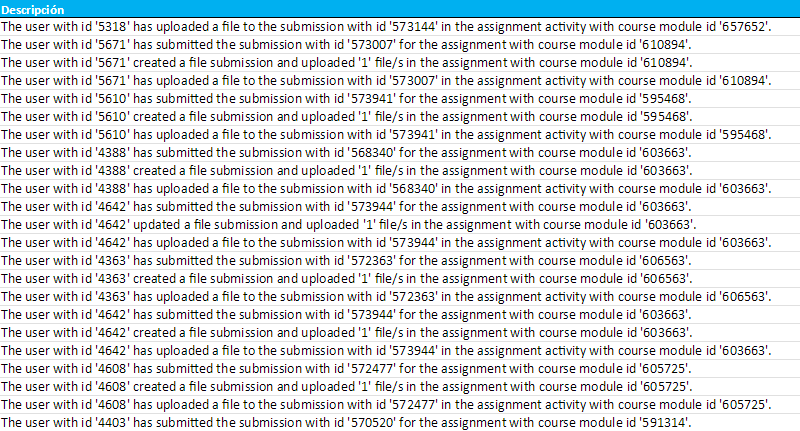
\includegraphics[width = 1 \textwidth]{Graphics/Pasted image 20240101131345.png}
        \caption{Campo descripción del archivo de registros de Moodle}
        \label{descrip}
    \end{figure} 
    
    \item \textbf{Transformación de datos}: La transformación de datos es el método de convertir datos de un formato a otro, generalmente del formato de un sistema origen al formato de un sistema destino. En este caso, se debe transformar el archivo de registros de Moodle a un formato que se adapte a las necesidades de los modelos de clasificación que se emplea. Un primer ejemplo, radica en el campo ``Descripción'' de este archivo de registros, que muestra su contenido como en la figura \ref{descrip}.  
    En la descripción aparece el id del estudiante, el id del módulo y en ocasiones, también el id del curso donde se está realizando la acción. Todo esto es información fundamental a la hora de organizar el \textit{dataset} que se desea obtener. El id del usuario se debe extraer para encontrar la calificación del mismo dentro del curso. Por otro lado, el id del módulo se extrae para saber a qué curso pertenece dicha acción. Por lo tanto, este campo se transforma en tres campos distintos por cada fila: el id del usuario, el id del módulo y el id del curso. Los mismos se obtuvieron con la utilización de expresiones regulares, que son cadenas de caracteres que permiten, a partir de un patrón en el texto, identificarlo y extraer la correspondiente información. 

    Una vez obtenidas estas nuevas columnas, agrupando por estudiante y luego por el curso, se obtienen todas las interacciones que posee un estudiante dentro de un curso determinado, y se empieza a contabilizar por cada uno de los atributos mencionados anteriormente correspondientes al \textit{dataset} que se desea formar. Además, para la predicción se convierten los valores numéricos de las calificaciones en valores binarios, de aprobado o no en el curso. Como se mencionó en el epígrafe 2.1, en este estudio se asume que un estudiante está desaprobado cuando tiene menos de 70 puntos y en caso contrario está aprobado.

    \item \textbf{Reducción de los datos}: La reducción de datos es la técnica que se emplea para obtener una representación reducida del conjunto manteniendo la integridad de los original de los mismos. En este estudio, por la cantidad de datos con los que se cuenta, no fue necesario realizar este paso.
    \item \textbf{Selección de características}: Una vez obtenidos los \textit{datasets}, se realizó un trabajo de selección de características dentro de los mismos. Con el objetivo de encontrar los atributos que más inciden en la predicción académica de un estudiante. 

    La selección de características es el proceso de escoger un subconjunto de atributos relevantes para construir modelos de aprendizaje robustos. Esta selección se clasifica en tres tipos: \textit{Wrapper}, \textit{Filter} e Híbridos. El primero emplea un algoritmo de aprendizaje automático para evaluar la fiabilidad de un conjunto de características; entre estos destacan dos algoritmos a mencionar: Boruta e Importancia de permutación (\textit{Permutation importance}). Mientras que el método \textit{Filter} utiliza las características de los datos para evaluar su importancia o rango por medida de distancia, medidas de correlación, medidas de consistencia y medida de información. Finalmente, los métodos Híbridos son una combinación de los dos anteriores, siendo útiles cuando existe un gran número de atributos para usar algoritmos del tipo \textit{Wrapper} y el rendimiento del enfoque basado en filtros no es satisfactorio. Este tipo de algoritmo pone en marcha un filtrado para medir la importancia de cada atributo.   
    
    Posteriormente, dentro del conjunto total se seleccionan diferentes subconjuntos de atributos y se evalúan desde el punto de vista de \textit{Wrapper}.
    En este estudio se utilizó el algoritmo Boruta [\cite{andreaperlato}] por su fácil manera de implementar. Es un algoritmo de tipo wrapper, el cual funciona extendiendo con otras acciones el \textit{Random Forest} y es capaz de trabajar con cualquier método de clasificación que pueda aplicar medidas de importancia de la variable. A continuación, se describe el funcionamiento del algoritmo:  


    


    \begin{enumerate}
        \item En la figura \ref{Boruta1} se observa que el algoritmo añade aleatoriedad al conjunto de datos al crear copias barajadas de un número determinado de características (denominadas características sombra u ocultas), por ejemplo, el atributo 1 con valores originales de 1 y 9, son asignados con valores sombra de 2 y 7. 
        
        \newpage
        \begin{figure}[htb]
            \centering
            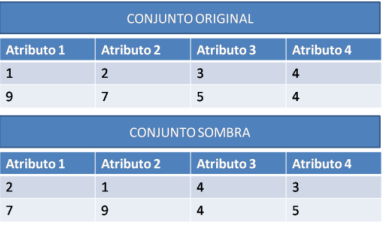
\includegraphics[width = 1 \textwidth]{Graphics/Pasted image 20240101133925.png}
            \caption{Conjunto de datos sombra y original (Descripción del algoritmo Boruta)}
            \label{Boruta1}
        \end{figure}
    
        \item El siguiente paso es entrenar un clasificador de \textit{Random Forest} en el conjunto de datos extendido y aplica una medida de importancia de la característica (el valor predeterminado es Precisión de disminución media) para evaluar la importancia de cada característica, cuando más reducción exista mayor significancia tendrá. 
        \item En cada iteración, verifica si una característica real tiene mayor importancia que la mejor de sus características sombra (es decir, si la característica tiene una puntuación Z más alta que la puntuación Z máxima de sus características sombra) y elimina constantemente las características que se consideran poco importantes. 
        \item Finalmente, el algoritmo se detiene cuando se confirman o rechazan todas las características o cuando alcanza un límite especificado de \textit{Decision Tree}.
    \end{enumerate}
\end{enumerate}

En este estudio se analizan el comportamiento de los modelos con los datasets originales y luego con los \textit{datasets} filtrados por las características relevantes encontradas por el algoritmo Boruta.

En el siguiente epígrafe se verán los modelos utilizados a profundidad.

\section{Análisis de modelos para la predicción}

Como se mencionó en el epígrafe anterior el proceso de investigación constó de 4 etapas, en este epígrafe se verá la propuesta de solución para la tercera y cuarta etapa.

\subsection{Construcción y entrenamiento de modelos de aprendizaje automático}

En este estudio se tuvo en cuenta cinco algoritmos de aprendizaje automático:

\begin{itemize}
    \item \textbf{Regresión Lineal}: es un método estadístico muy utilizado en técnicas de \textit{Machine Learning}. Estas estimaciones de regresión explican la correlación entre las variables dependientes e independientes. La forma más simple de la regresión se define mediante la siguiente ecuación:
    \begin{center}
        $Y = \beta_0 + \beta_1X + \epsilon$
    \end{center}
    donde $\beta_0, \beta_1 \in \mathbb{R}$ son constantes desconocidas llamadas coeficientes de regresión, las cuales se pueden calcular como estimaciones de algunos parámetros del modelo, definiendo la relación entre dos entidades (valor del predictor y respuesta). Hay tres tipos principales de análisis de regresión, que incluyen pronosticar un efecto, determinar la fuerza de los predictores y pronosticar tendencias. [\cite{faul2019concise}]
    \item \textbf{Regresión logística}: es un tipo de análisis de clasificación utilizado para predecir el resultado de una variable categórica (una variable que puede adoptar un número limitado de categorías) en función de las variables independientes o predictoras. Es útil para modelar la probabilidad de un evento ocurriendo en función de otros factores, en el caso que ocupa este trabajo puede ser: si un estudiante aprobó o no. Este algoritmo puede manejar no sólo el ajuste de una línea de regresión sino también el ajuste de un método logístico en forma de ``S'' que predice dos estados máximos (0 o 1). [\cite{wei-meng2019python}]
    \item \textbf{Árbol de decisión}: es una de las técnicas de aprendizaje más efectivas y ampliamente utilizada en diversas áreas como educación, estadística, banca y reconocimiento, entre otras. La estructura del árbol se construye a partir de un nodo raíz, nodos internos y nodos hoja. Cada nodo se puede definir como el momento en el que se ha de tomar una decisión de entre varias posibles, lo que va haciendo que a medida que aumenta el número de nodos aumente el número de posibles finales a los que se puede llegar. El algoritmo prueba un atributo en todos los nodos internos, la salida de la prueba está en una rama, mientras que a cada nodo hoja se le asigna una etiqueta de clase, es decir, la clasificación a la que se desea llegar. [\cite{faul2019concise}]
    \item \textit{\textbf{Random Forest}}: es un método de aprendizaje automático supervisado de uso común que desempeña un papel importante en los problemas de clasificación y regresión. Es un grupo de árboles de decisión, pero en este caso solo se seleccionan un subconjunto de características, mientras que el árbol de decisión considera todas las posibles divisiones de atributos. El algoritmo presenta características claves, como producir una predicción razonable sin ajuste de hiperparámetros, reduce el riesgo de sobre ajuste, proporciona flexibilidad y determina fácilmente la importancia de las características. [\cite{faul2019concise}]
    \item \textit{\textbf{Support Vector Machine (SVM)}}: es un método de aprendizaje supervisado adaptable para problemas que involucran clasificación y regresión. Cada punto de datos en un espacio de $n$ dimensiones corresponde al valor de cada atributo. Luego, la clasificación se realiza seleccionando el hiperplano que mejor distingue las dos clases. SVM puede realizar una clasificación lineal de manera eficiente al \textit{mapear} el conjunto de entrada dado en espacios de dimensiones superiores. Se agrupa en dos tipos diferentes, SVM lineal y no lineal. [\cite{wei-meng2019python}]
\end{itemize}

El proceso de construcción y entrenamiento se dividió en tres etapas:
\begin{enumerate}
    \item Los datos recopilados y ya procesados se dividieron en dos conjuntos, con el 80\% el primer conjunto sirviendo como datos de entrenamiento y el 20\% restante como datos de prueba.
    \item Se seleccionaron los 5 algoritmos basados en los más utilizados para la clasificación (\textit{Random Forest}, Árbol de decisión, Regresión lineal, Regresión logística, \textit{Support Vector Machine}).
    \item Entrenamiento y evaluación de los modelos seleccionados.
\end{enumerate}

\subsection{Evaluación}

El experimento se dividió en dos pasos para la fase de evaluación del modelo: validación cruzada de k veces y evaluación del modelo.  

\begin{enumerate}
    \item Se evaluaron los 5 clasificadores mediante validación cruzada quíntuple, una de las técnicas más utilizadas para medir un modelo en \textit{Machine Learining} (Aprendizaje de máquina). En este paso el conjunto de entrenamiento en cada iteración de la validación cruzada se dividió nuevamente en el 80\% para el entrenamiento y el 20\% para la validación. Por lo tanto se construyó un modelo compuesto por cinco iteraciones, donde, en cada iteración se utilizaron conjuntos de validación y entrenamiento diferentes.
    \item Se evaluó el rendimiento de los modelos calculando la puntuación de rendimiento promedio de todos los k pasos. Cada etapa del curso (25\%, 50\%, 75\% y 100\%), se le aplicó el enfoque mencionado de la misma manera.
\end{enumerate}

La evaluación del desempeño se realizó con la Matriz de Confusión con dos etiquetas de clase, ampliamente utilizada para la evaluación de la calidad de la clasificación [\cite{faul2019concise}]. Se utilizaron una variedad de cuatro medidas comunes: exactitud, precisión, recuperación y medida F1 [\cite{rehman2019automatic}].

Sean:  
\begin{itemize}
    \item $TP$ = Verdadero Positivo (predicho verdadero y verdadero en la realidad)
    \item $TN$ = Verdadero Negativo (predicho falso y falso en realidad)
    \item $FP$ = Falso Positivo (predicho verdadero y falso en realidad)
    \item $FN$ = Falso Negativo (predicho falso y verdadero en la realidad)
\end{itemize}

Cada métrica está definida de la siguiente manera:  
\begin{itemize}
    \item \textbf{Exactitud}: se define como la proporción entre el número total de clasificaciones correctas y el total de clasificaciones.
    \begin{center}
        $Exactitud = \frac{TP + TN}{TP + TN + FP+ FN} $
    \end{center}
    \item \textbf{Precisión}: es la proporción de casos de predicción positivos que se clasifican correctamente. 
    \begin{center}
        $Precision = \frac{TP}{TP + FP}$
    \end{center}
    \item \textbf{Recuperación}: es la proporción de casos de predicción realmente positivos que se clasificaron correctamente. 
    \begin{center}
        $Recuperacion = \frac{TP}{TP+FN}$
    \end{center}
    \item \textbf{Medida F1}: es la media armónica entre la precisión y la recuperación. Sus valores oscilan entre 0 y 1, mientras más cercano a 1 sea su valor mejor es el clasificador. 
    \begin{center}
        $$F1 = \frac{2 * Precision * Recuperacion}{Precision + Recuperacion}$$
    \end{center}

\end{itemize}

En el siguiente capítulo se aborda con más detalle la implementación y los resultados de todo el proceso de investigación.  



\chapter{Detalles de Implementación y Experimentos}\label{chapter:implementation}


\backmatter

\begin{conclusions}
    Conclusiones  

    Como resultado del presente trabajo se logró la creación de una solución computacional que responde a la problemática de predicción académica, en la que se integran 
    técnicas estadísticas, de análisis de datos y de aprendizaje automático. La solución se caracteriza por la construcción de modelos de datos educacionales y de aprendizaje automático con vista a favorecer el análisis descriptivo del comportamiento de un estudiante dentro de un curso virtual, así como 
    el uso de las potencialidades que brinda una LMS como Moodle.  

    A partir de la profundización en las áreas de conocimiento asociadas, el acercamiento al contexto educativo y 
    el estudio de soluciones similares a la predicción del desempeño académico. Se logró el diseñó de una metodología general para el procesamiento de datos educacionales de la plataforma Moodle, a partir de la cual, se implementó un prototipo sobre cuya base se aplicó un conjunto de experimentos que 
    permitió establecer la validez de la concepción global.  

    La creación de una solución computacional basada en los avances científicos y tecnológicos para el análisis de los datos históricos de los estudiantes, la construcción de diferentes conjuntos de datos con distintos atributos implicados, la selección de características dentro de estos, el procesamiento del lenguaje natural a la hora de limpiar los datos, así como realizar la predicción en las diferentes etapas del curso 
    constituyen aportes con respecto a las herramientas o soluciones computacionales implementadas con anterioridad en el ámbito de la analítica del aprendizaje.  
    
    Los resultados de la investigación permiten responder afirmativamente a la pregunta científica, ya que ha sido posible la predicción del desempeño estudiantil a partir de modelos de aprendizaje automático, incorporando nuevas formas del procesamiento de los datos de Moodle. 

    
\end{conclusions}

\begin{recomendations}
    \begin{itemize}
        \item Contribuir a la evolución de esta investigación con una herramienta que automatice todos los procesos: preprocesamiento de datos de Moodle para la posterior predicción. 
        \item Realizar el entrenamiento de los modelos con un cojunto de datos más grande con el objetivo de lograr mayor robustez en los algoritmos empleados. 
        \item Incorporar nuevos modelos (redes neuronales), así como, otros enfoques, como el de aprendizaje no supervisado.
        \item Mejorar el empleo de las plataformas por parte de los profesores y estudiantes, con el objetivo de obtener datos más correspondientes con la realidad del curso virtual en cuestión.
        \item Implementar un sistema de recomendaciones en el Entorno Virtual de Aprendizaje que facilite la retroalimentación de los estudiantes en aras de mejorar su desempeño partiendo de las predicciones que se tengan de cada estudiante o de cada curso.
    \end{itemize}


\end{recomendations}

\printbibliography[heading=bibintoc]


\end{document}